\documentclass[12pt,a4paper,fleqn]{article}
\title{Progress Report}
\author{Syed Ahmad Raza}
\date{2018.05.30}
\usepackage{mathtools}      % for math
\usepackage{graphicx}       % for graphics
%\usepackage{xcolor}         % for using colors in document
%\usepackage{afterpage}
\usepackage{float}          % force a figure placement with [H] command
%\usepackage{enumitem}       % control layout of itemize and enumerate
\usepackage{newtxtext}      % better text font
\usepackage{newtxmath}      % better math font
\usepackage{nicefrac}       % use nicer smaller fractions
%\usepackage{layouts}       % find \printinunitsof{in}\prntlen{\textwidth}
\graphicspath{{../figures/}}% only works when -shell-escape option is used

\begin{document}
\maketitle
%\tableofcontents
%\pagebreak

\section{First results for 3D Navier-Stokes Solver}

A three-dimensional finite volume Navier-Stokes solver was coded in C++. The results for QUICK scheme using a course 11\(\times\)11\(\times\)11 grid size are shown in the figures below.

\begin{figure}[H]
    \centering
    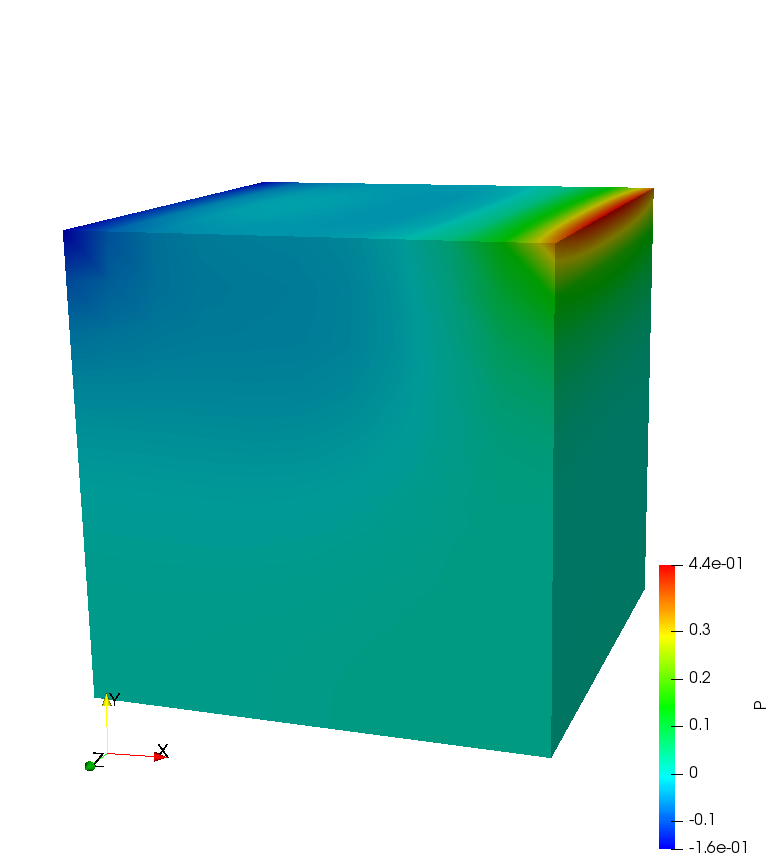
\includegraphics[width=\linewidth]{3d_quick_pressure.png}
    \caption{Pressure contours for three-dimensional cavity flow}
\end{figure}

\begin{figure}[H]
    \centering
    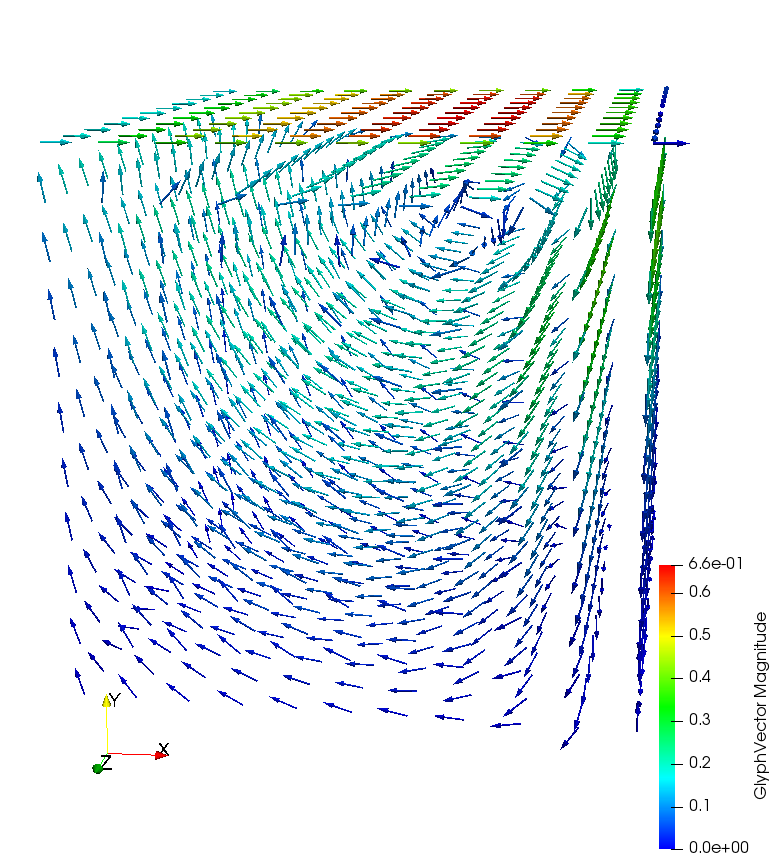
\includegraphics[width=\linewidth]{3d_quick_velVectors.png}
    \caption{Velocity vectors for three-dimensional cavity flow}
\end{figure}

\subsection{Future tasks}
\begin{enumerate}
    \item Converting the code for use with parallel computing using OpenMP
    \item Obtain and analyze the results for larger grid sizes
    \item Validate the 3D code using results from published literature
\end{enumerate}

\end{document}
